\section{Stoffklassen}
    % Stoffe lassen sich in 3 Arten einteilen:
    \begin{itemize}
        \item \textbf{molekulare Stoffe \& Edelgase:}
        \begin{itemize}
            \item Abgeschlossener Atomverband aus Nichtmetallen (Molekül)
            \item \tikz[baseline=(text.base)]\node[fill=green, fill opacity=0.3, text opacity=1, rounded corners, inner sep=2pt, minimum height=5pt] (text) {Formel:}; genaue Anzahl Atome pro Molekül, z.B \ce{H_2O} oder \ce{He}
            \item Nicht elektrisch Leitend, da keine freien Ladungsträger vorhanden
        \end{itemize}
        \item \textbf{Metalle und Halbmetalle:}
        \begin{itemize}
            \item unendlicher Verband aus metallischen Atomkernen umgeben von delokaliserten (Valenz-) Elektronen (Elektronen-Wolke)
            \item \tikz[baseline=(text.base)]\node[fill=green, fill opacity=0.3, text opacity=1, rounded corners, inner sep=2pt, minimum height=5pt] (text) {Formel:}; Verhältnis der Atome im Gitter. Z.B. \ce{Fe}
        \end{itemize}
        \item \textbf{Salze:}
        \begin{itemize}
            \item unendl. Verband aus metallischen Kationen(\ce{+}) und nichtmetall. Anionen(\ce{-}) 
            
                (können auch molekulare Kationen sein(\ce{SO4-}))

            \item \tikz[baseline=(text.base)]\node[fill=green, fill opacity=0.3, text opacity=1, rounded corners, inner sep=2pt, minimum height=5pt] (text) {Formel:}; Verhältnis der Kationen und Anionen, z.B. \ce{Al_2O_3} = \ce{Al^{3+} und \ce{O^{2-}}}
            \item Besitzt in Schmelze und in Lösung freie Ladungsträger (Ionen) 
            
                $\rightarrow$ leitet in diesen Zuständen dementsprechend gut Strom
        \end{itemize}
    \end{itemize}
\subsection{Metalle und Halbmetalle}
    Metalle besitzen durch delokalisierte Ve (Elektronenwolke) freie Ladungsträger 
    \begin{itemize}
        \item[$\rightarrow$] gute Wärme- und el. Leitfähigkeit, Verformbarkeit
        \item Leitfähigkeit bei Metallen
        \begin{itemize}
            \item nimmt mit steigender Temperatur ab
            
                $\rightarrow$ Die Bewegung der Atomrümpfe erhöht sich
                
                $\Rightarrow$ weniger Platz für die Elektronenbewegung
        \end{itemize}
    \end{itemize}
    \begin{minipage}{0.48\columnwidth}
        \textbf{Beispiel Lithium:}
            \begin{itemize}
                \item Valenzband (spez. Energieniveau) nicht ganz gefüllt
                
                    $\rightarrow$ Elektronen können sich im Band bewegen
            \end{itemize}
    \end{minipage}
    \hfill
    \begin{minipage}{0.48\columnwidth}
        \textbf{Beispiel Beryllium:}
            \begin{itemize}
                \item Valenzband komplett gefüllt, aber mit leerem Leitungsband überlappend
                
                    $\rightarrow$ Elektronen können sich im Band bewegen
            \end{itemize} 
    \end{minipage}
    \begin{center}
        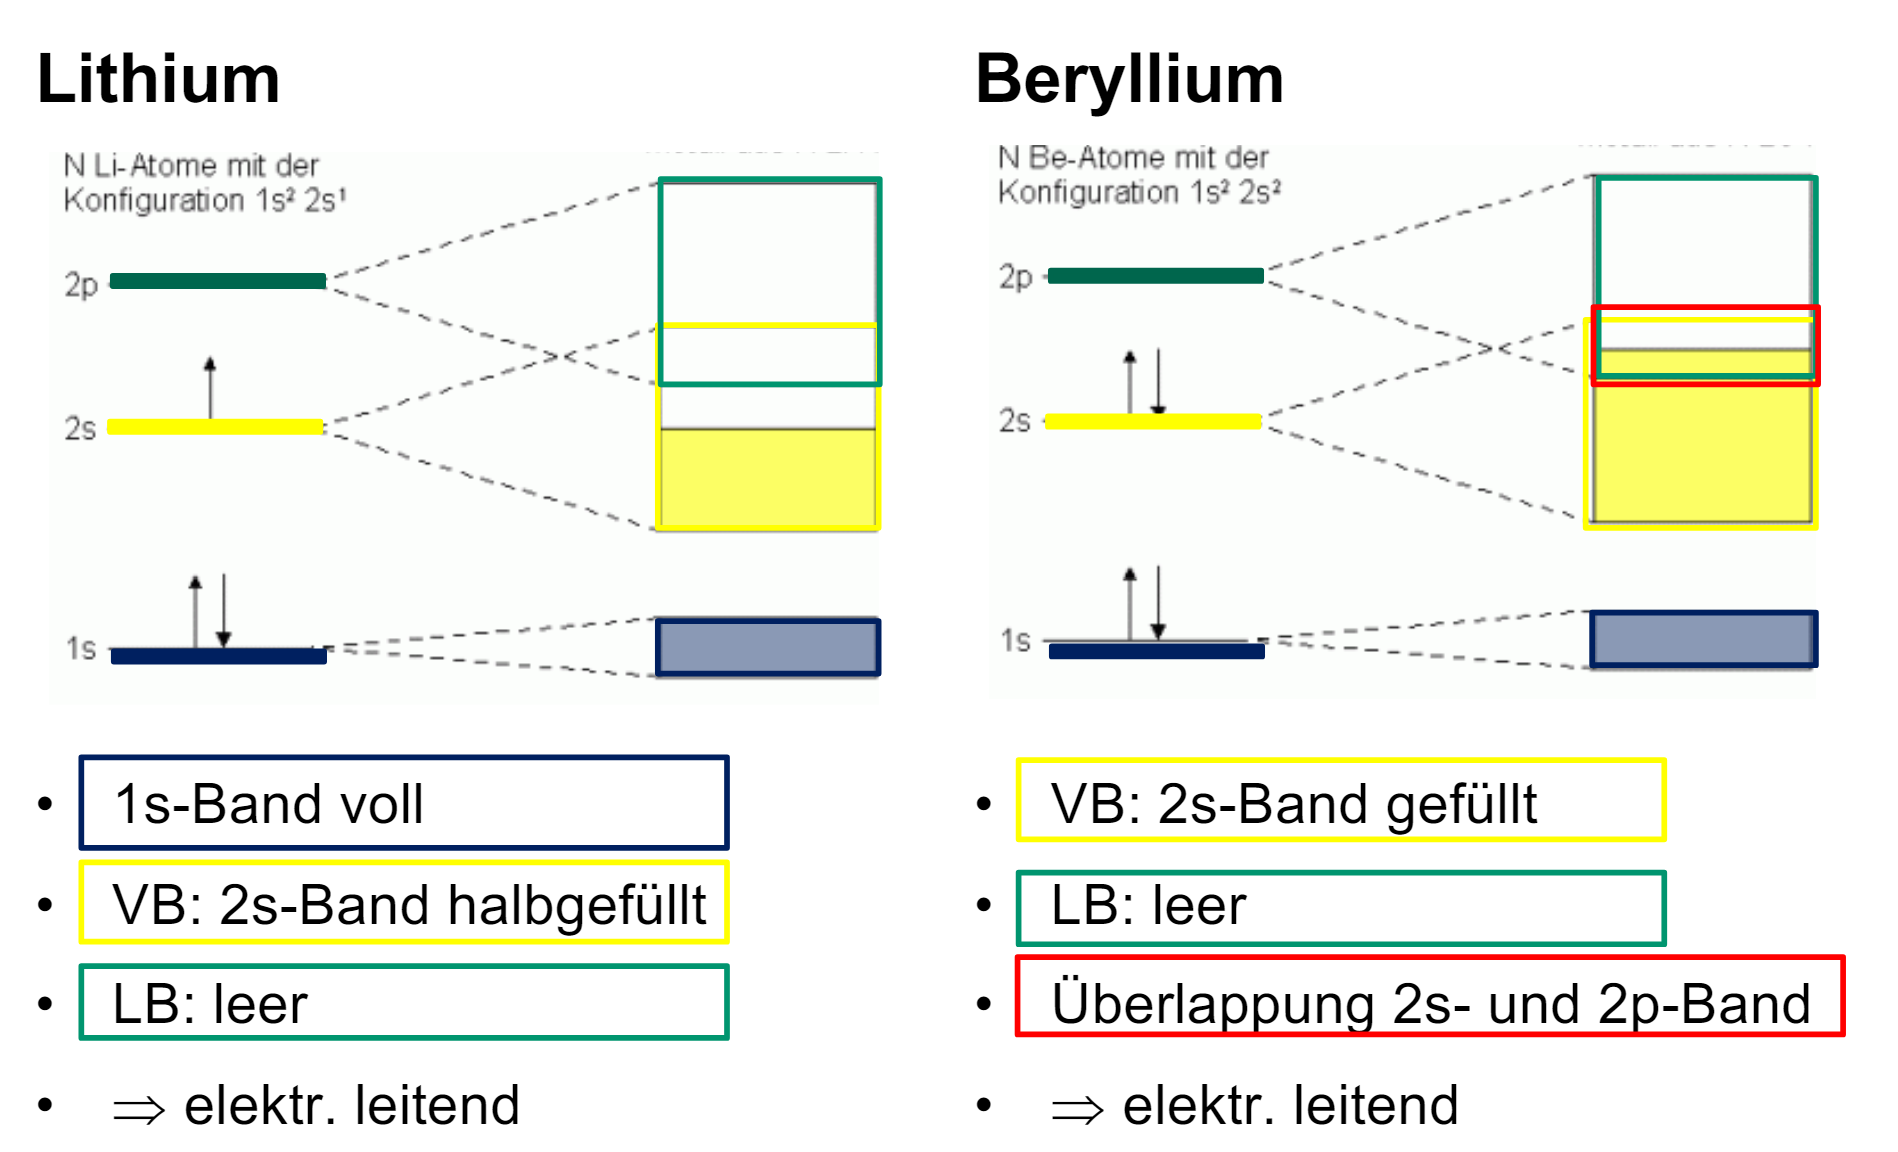
\includegraphics[height=3cm]{pictures/Baender.png}
    \end{center}
    Halbmetalle haben weder Elektronenwolken noch überlappende Energieniveaus, Nähe vom Valenz- und Leitungsband ermöglichen aber ein Überspringen
    \begin{itemize}
        \item Leitfähigkeit bei Halbmetallen 
        \begin{itemize}
            \item nimmt mit steigender Temperatur stark zu
            
                $\rightarrow$ Die Elektronen springen viel zahlreicher auf das Leitungband über
                
                $\Rightarrow$ Platz für Elektronenbewegung im Leitungsband
        \end{itemize}
    \end{itemize}
    % Metalle besitzen durch delokal. Ve (Elektronenwolke) freie Ladungsträger $\rightarrow$ gute Wärme- und el. Leitfähigkeit, Verformbarkeit
    % \begin{itemize}
    %     \item Leitfähigkeit nimmt mit steigender Temperatur ab.\\Die Bewegung der Atomrümpfe erhöht sich wodurch weniger Platz für die ELektronen um sich zu bewegen bleibt.
    % \end{itemize}
    % Allgemein sind Stoffe leitfähig wenn sie entweder wie Lithium:
    % \begin{itemize}
    %     \item das Valenzband (spez. Energieniveau) nicht ganz gefüllt haben und sich dadurch ELektronen in jenem Band bewegen können.
    % \end{itemize}
    % oder wenn sie wie Beryllium:
    % \begin{itemize}
    %     \item das Valenzband komplett gefüllt haben dieses jedoch mit einem leeren Leitungsband überlappt. Wodurch wiederum die beweglichkeit der Elektronen gewährleistet ist.
    % \end{itemize}
    % Halbmetalle haben weder Elektronenwolken noch überlappende Energieniveaus jedoch sind Valenz- und Leitungsband so nahe bei einander das ein überspringen ermöglicht wird.
    % \begin{itemize}
    %     \item Leitfähigkeit nimmt mit zunehmender Temperatur stark zu.\\Die Elektronen springen viel zahlreicher auf das Leitungband über wodurch im Leitungsband wiederum Platz für Elektronenbewegung geschaffen wird.
    % \end{itemize}

\subsection{Dotierung von Halbmetallen}
    Dotierung $\rightarrow$ Einbringen von Fremdatomen ins Atomgitter eines Halbleiters
    \begin{itemize}
        \item \textbf{n-Halbleiter}
        \item[] z.B. einzelne As-Atome im Si-Gitter(1:10'000'000)
        \item[] Ein \tikz[baseline=(text.base)]\node[fill=orange, fill opacity=0.3, text opacity=1, rounded corners, inner sep=2pt, minimum height=5pt] (text) {\textit{überschüssiges}}; 
        Elektron pro As-Atom $\Rightarrow$ Leitfähigkeit: Elektron von As-Atom kann ins Leitungsband von Si überspringen und sich frei bewegen
        \item \textbf{p-Halbleiter}
        \item[] z.B. einzelne B-Atome im Si-Gitter(1:1'000'000)
        \item[] Ein \tikz[baseline=(text.base)]\node[fill=orange, fill opacity=0.3, text opacity=1, rounded corners, inner sep=2pt, minimum height=5pt] (text) {\textit{fehlendes}}; Elektron pro B-Atom $\Rightarrow$ Leitfähigkeit: Elektronen aus dem vollen Valenzband von Si können in diese ``Lücke'' springen und sich frei bewegen
    \end{itemize}
\subsection{Bindungswinkel}
    \begin{center}
    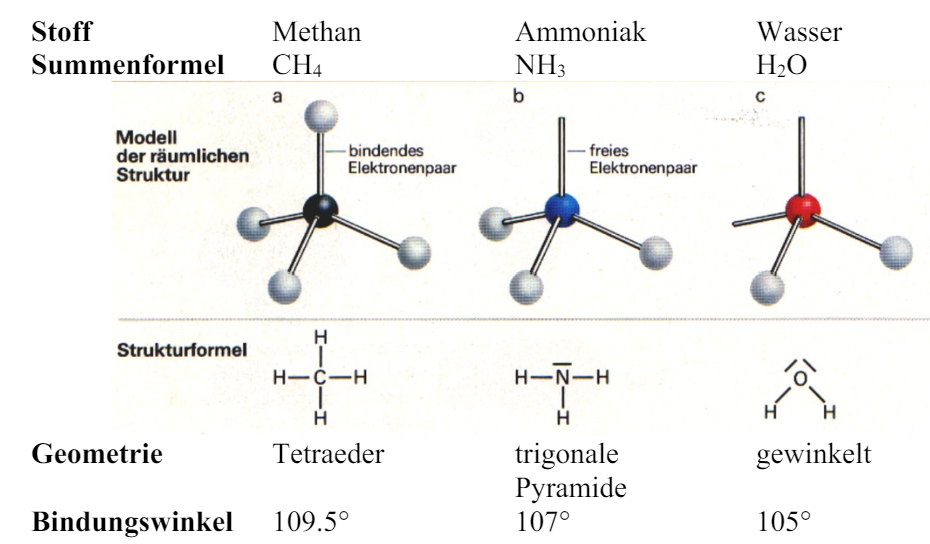
\includegraphics[height=4cm]{pictures/Winkel.png}
    \end{center}

\subsection{Zwischenmolekularkräfte ZMK}
    \begin{itemize}
        \item ... beinflussen Schmelzp., Siedep., Löslichkeit, Viskosität, Oberflächenspannung, ...
        \begin{itemize}
            \item Van der Waals (asymm. $e^-$-Verteilung, abh. Anzahl $e^-$) \textcolor{red}{sehr schwach}
            \item Dipol-Dipol (Partialladung, $\delta^+, \delta^-$, $\Delta$EN) \textcolor{orange}{schwach}
            \item Wasserstoffbrücken (H-F-, H-O- oder H-N-Bindungen) \textcolor{green!80!black}{stark}
        \end{itemize}
    \end{itemize}

\subsection{Löslichkeit}
    Die Löslichkeit von Salzen hängt von ihrer Bildungsstärke ab. Je grösser die Ladung der Ionen und je grösser die Ionen, desto schlechter sind sie in Wasser löslich.
    
    \begin{minipage}{0.49\columnwidth}
        \textbf{Immer gut löslich sind:}
        \begin{itemize}
            \item \textbf{alle} Alkalisalze (\ce{NaCl, KOH, ...})
            \item \textbf{alle} Ammoniumsalze (\ce{NH4Cl, ...})
            \item \textbf{alle} Nitratsalze (\ce{Pb(NO3)2, Ca(NO3)2})
            \item \textbf{alle} Hydrogensalze (\ce{Ca(HCO3)2})
        \end{itemize}
    \end{minipage}
    \hfill
    \begin{minipage}{0.49\columnwidth}
        \textbf{Oft schwer löslich sind:}
        \begin{itemize}
            \item \textbf{viele} Sulfidsalze (\ce{PbS, ...})
            \item \textbf{viele} Phosphatsalze (\ce{AlPO4, ...})
            \item \textbf{viele} Carbonatsalze (\ce{CaCO3, ...})
            \item \textbf{viele} Erdalkalisalze (\ce{MgCl2, ...})
        \end{itemize}
    \end{minipage}
    
    % \begin{center}
    %     \includegraphics[height=2cm]{pictures/Löslichkeit.png}
    % \end{center}